\documentclass[aspectratio=169,10pt]{beamer}
\usetheme[progressbar=frametitle,numbering=fraction]{metropolis}
\usefonttheme{professionalfonts}
\usepackage[T1]{fontenc}
\usepackage{sourcesanspro}
\usepackage{booktabs}
\usepackage{tikz}
\usetikzlibrary{arrows.meta,positioning,shapes.geometric}
\newcommand{\NumCaptures}{144}
\newcommand{\NumQASamples}{16}
\newcommand{\NumSummarySamples}{8}
\newcommand{\QATwoUploadReductionTLS}{54}
\newcommand{\QAFourUploadReductionTLS}{76}
\newcommand{\QATwoTotalReductionTLS}{51}
\newcommand{\QAFourTotalReductionTLS}{71}
\newcommand{\SummaryTwoUploadReductionTLS}{38}
\newcommand{\SummaryFourUploadReductionTLS}{55}
\newcommand{\SummaryTwoTotalReductionTLS}{6}
\newcommand{\SummaryFourTotalReductionTLS}{20}
\newcommand{\TokenUploadCorrelationTLS}{0.88}
\newcommand{\TokenUploadCorrelationQUIC}{0.88}

\usepackage{pgfplots}
\usepgfplotslibrary{groupplots,statistics,fillbetween}
\pgfplotsset{compat=1.18}

\definecolor{AIBlue}{HTML}{0072B2}
\definecolor{AIOrange}{HTML}{D55E00}
\definecolor{AIGreen}{HTML}{009E73}
\definecolor{AIPurple}{HTML}{7B61A8}
\definecolor{AIGray}{HTML}{6B7280}
\definecolor{AIGrid}{HTML}{E5E7EB}

\pgfplotsset{
  conference/.style={
    width=0.93\linewidth,
    height=0.56\textheight,
    axis line style={draw=AIGray},
    tick style={draw=AIGray},
    grid=major,
    grid style={draw=AIGrid,line width=0.35pt},
    tick label style={font=\scriptsize},
    label style={font=\small},
    title style={font=\small\bfseries},
    legend style={
      draw=none,
      fill=none,
      font=\scriptsize,
      /tikz/every even column/.append style={column sep=0.8em}
    },
    every axis plot/.append style={line width=1.2pt},
    unbounded coords=discard,
  },
  conference bar/.style={
    conference,
    ybar,
    bar width=8pt,
    enlarge x limits=0.22,
    nodes near coords,
    nodes near coords style={font=\tiny,/pgf/number format/fixed,/pgf/number format/precision=0},
    legend columns=-1,
  },
}

\newcommand{\PlotTokenMedians}{
\begin{tikzpicture}
\begin{axis}[
  conference bar,
  xtick={0,1,2},
  xticklabels={Original,2x,4x},
  ylabel={Median input tokens (thousands)},
  ymin=0,
  ymax=52,
  legend style={at={(0.5,1.02)},anchor=south,legend columns=-1},
]
\addplot+[fill=AIBlue,draw=AIBlue] table[x=x,y=qa_k,col sep=comma]
  {figures/data/plot_token_medians.csv};
\addplot+[fill=AIOrange,draw=AIOrange] table[x=x,y=summary_k,col sep=comma]
  {figures/data/plot_token_medians.csv};
\legend{QA,Event summary}
\end{axis}
\end{tikzpicture}
}

\newcommand{\ReductionPlot}[2]{
\begin{tikzpicture}
\begin{groupplot}[
  group style={group size=2 by 1,horizontal sep=1.25cm},
  conference bar,
  width=0.46\linewidth,
  height=0.54\textheight,
  xtick={0,1},
  xticklabels={2x,4x},
  ylabel={Median reduction (\%)},
  ymin=0,
  ymax=85,
  legend style={at={(0.5,1.16)},anchor=south,legend columns=-1},
  error bars/y dir=both,
  error bars/y explicit,
]
\nextgroupplot[title={QA}]
\addplot+[fill=AIBlue,draw=AIBlue] table[
  x=x,y=qa_tls13,y error plus=qa_tls13_err_plus,y error minus=qa_tls13_err_minus,col sep=comma]
  {#1};
\addplot+[fill=AIOrange,draw=AIOrange] table[
  x=x,y=qa_http3,y error plus=qa_http3_err_plus,y error minus=qa_http3_err_minus,col sep=comma]
  {#1};
\legend{TLS 1.3,HTTP/3}
\nextgroupplot[title={Event summary},ylabel={}]
\addplot+[fill=AIBlue,draw=AIBlue] table[
  x=x,y=summary_tls13,y error plus=summary_tls13_err_plus,y error minus=summary_tls13_err_minus,col sep=comma]
  {#1};
\addplot+[fill=AIOrange,draw=AIOrange] table[
  x=x,y=summary_http3,y error plus=summary_http3_err_plus,y error minus=summary_http3_err_minus,col sep=comma]
  {#1};
\end{groupplot}
\end{tikzpicture}
}
\newcommand{\PlotUploadReduction}{
  \ReductionPlot{figures/data/plot_upload_reduction.csv}{Client-to-server bytes}
}
\newcommand{\PlotTotalReduction}{
  \ReductionPlot{figures/data/plot_total_reduction.csv}{Bidirectional frame bytes}
}
\newcommand{\PlotLatencyReduction}{
  \ReductionPlot{figures/data/plot_latency_reduction.csv}{End-to-end generation latency}
}

\newcommand{\DirectionPlot}[2]{
\begin{tikzpicture}
\begin{axis}[
  conference,
  ybar stacked,
  bar width=15pt,
  width=0.96\linewidth,
  height=0.56\textheight,
  xtick={0,1,2,4,5,6},
  xticklabels={TLS Orig.,TLS 2x,TLS 4x,H3 Orig.,H3 2x,H3 4x},
  xticklabel style={rotate=22,anchor=east,font=\scriptsize},
  ylabel={Median captured bytes (KiB)},
  ymin=0,
  legend style={at={(0.5,1.02)},anchor=south,legend columns=-1},
]
\addplot+[fill=AIBlue,draw=AIBlue] table[x=x,y=upload_kib,col sep=comma]{#1};
\addplot+[fill=AIOrange,draw=AIOrange] table[x=x,y=download_kib,col sep=comma]{#1};
\legend{Client $\rightarrow$ server,Server $\rightarrow$ client}
\end{axis}
\end{tikzpicture}
}
\newcommand{\PlotDirectionQA}{
  \DirectionPlot{figures/data/plot_direction_qa.csv}{QA is upload dominated}
}
\newcommand{\PlotDirectionSummary}{
  \DirectionPlot{figures/data/plot_direction_summary.csv}{Summary traffic is output dominated}
}

\newcommand{\PlotProtocolBytes}{
\begin{tikzpicture}
\begin{axis}[
  conference bar,
  xtick={0,1,2},
  xticklabels={Original,2x,4x},
  ylabel={HTTP/3 / TLS total-byte ratio},
  ymin=0.85,
  ymax=1.12,
  nodes near coords style={font=\tiny,/pgf/number format/fixed,/pgf/number format/precision=2},
  legend style={at={(0.5,1.02)},anchor=south,legend columns=-1},
]
\addplot+[fill=AIBlue,draw=AIBlue] table[x=x,y=qa_bytes,col sep=comma]
  {figures/data/plot_protocol_ratio.csv};
\addplot+[fill=AIOrange,draw=AIOrange] table[x=x,y=summary_bytes,col sep=comma]
  {figures/data/plot_protocol_ratio.csv};
\addplot[AIGray,dashed,sharp plot,forget plot] coordinates {(-0.5,1) (2.5,1)};
\legend{QA,Event summary}
\end{axis}
\end{tikzpicture}
}

\newcommand{\PlotProtocolPackets}{
\begin{tikzpicture}
\begin{axis}[
  conference bar,
  xtick={0,1,2},
  xticklabels={Original,2x,4x},
  ylabel={HTTP/3 / TLS packet-count ratio},
  ymin=0,
  ymax=3.3,
  nodes near coords style={font=\tiny,/pgf/number format/fixed,/pgf/number format/precision=2},
  legend style={at={(0.5,1.02)},anchor=south,legend columns=-1},
]
\addplot+[fill=AIBlue,draw=AIBlue] table[x=x,y=qa_packets,col sep=comma]
  {figures/data/plot_protocol_ratio.csv};
\addplot+[fill=AIOrange,draw=AIOrange] table[x=x,y=summary_packets,col sep=comma]
  {figures/data/plot_protocol_ratio.csv};
\addplot[AIGray,dashed,sharp plot,forget plot] coordinates {(-0.5,1) (2.5,1)};
\legend{QA,Event summary}
\end{axis}
\end{tikzpicture}
}

\newcommand{\PlotLatencyMedians}{
\begin{tikzpicture}
\begin{groupplot}[
  group style={group size=2 by 1,horizontal sep=1.2cm},
  conference,
  width=0.46\linewidth,
  height=0.54\textheight,
  xtick={0,1,2},
  xticklabels={Original,2x,4x},
  ylabel={Median latency (s)},
  ymin=0,
  legend style={at={(0.5,1.16)},anchor=south,legend columns=-1},
]
\nextgroupplot[title={QA},ymax=10]
\addplot+[mark=*,color=AIBlue] table[x=x,y=qa_tls13,col sep=comma]{figures/data/plot_latency_medians.csv};
\addplot+[mark=square*,color=AIOrange] table[x=x,y=qa_http3,col sep=comma]{figures/data/plot_latency_medians.csv};
\legend{TLS 1.3,HTTP/3}
\nextgroupplot[title={Event summary},ylabel={},ymax=28]
\addplot+[mark=*,color=AIBlue] table[x=x,y=summary_tls13,col sep=comma]{figures/data/plot_latency_medians.csv};
\addplot+[mark=square*,color=AIOrange] table[x=x,y=summary_http3,col sep=comma]{figures/data/plot_latency_medians.csv};
\end{groupplot}
\end{tikzpicture}
}

\newcommand{\PlotAbsoluteTotal}{
\begin{tikzpicture}
\begin{groupplot}[
  group style={group size=2 by 1,horizontal sep=1.2cm},
  conference bar,
  width=0.46\linewidth,
  height=0.54\textheight,
  xtick={0,1,2},
  xticklabels={Original,2x,4x},
  ylabel={Median total traffic (KiB)},
  ymin=0,
  legend style={at={(0.5,1.16)},anchor=south,legend columns=-1},
]
\nextgroupplot[title={QA},ymax=180]
\addplot+[fill=AIBlue,draw=AIBlue] table[x=x,y=qa_tls13,col sep=comma]{figures/data/plot_total_kib.csv};
\addplot+[fill=AIOrange,draw=AIOrange] table[x=x,y=qa_http3,col sep=comma]{figures/data/plot_total_kib.csv};
\legend{TLS 1.3,HTTP/3}
\nextgroupplot[title={Event summary},ylabel={},ymax=430]
\addplot+[fill=AIBlue,draw=AIBlue] table[x=x,y=summary_tls13,col sep=comma]{figures/data/plot_total_kib.csv};
\addplot+[fill=AIOrange,draw=AIOrange] table[x=x,y=summary_http3,col sep=comma]{figures/data/plot_total_kib.csv};
\end{groupplot}
\end{tikzpicture}
}

\newcommand{\PlotTokenUploadScatter}{
\begin{tikzpicture}
\begin{groupplot}[
  group style={group size=2 by 1,horizontal sep=1.2cm},
  conference,
  width=0.46\linewidth,
  height=0.54\textheight,
  xlabel={Input tokens},
  ylabel={Client-to-server traffic (KiB)},
  xmin=0,
  ymin=0,
  legend style={at={(0.5,1.16)},anchor=south,legend columns=-1},
]
\nextgroupplot[title={TLS 1.3}]
\addplot+[only marks,mark=*,mark size=1.7pt,color=AIBlue,opacity=0.72]
  table[x=input_tokens,y=upload_kib,col sep=comma]{figures/data/scatter_qa_tls13.csv};
\addplot+[only marks,mark=triangle*,mark size=2pt,color=AIOrange,opacity=0.72]
  table[x=input_tokens,y=upload_kib,col sep=comma]{figures/data/scatter_summary_tls13.csv};
\legend{QA,Event summary}
\nextgroupplot[title={HTTP/3},ylabel={}]
\addplot+[only marks,mark=*,mark size=1.7pt,color=AIBlue,opacity=0.72]
  table[x=input_tokens,y=upload_kib,col sep=comma]{figures/data/scatter_qa_http3.csv};
\addplot+[only marks,mark=triangle*,mark size=2pt,color=AIOrange,opacity=0.72]
  table[x=input_tokens,y=upload_kib,col sep=comma]{figures/data/scatter_summary_http3.csv};
\end{groupplot}
\end{tikzpicture}
}

\newcommand{\PlotTotalECDF}{
\begin{tikzpicture}
\begin{groupplot}[
  group style={group size=2 by 1,horizontal sep=1.2cm},
  conference,
  width=0.46\linewidth,
  height=0.54\textheight,
  xlabel={Compressed / original total bytes},
  ylabel={Fraction of paired samples},
  xmin=0.2,
  xmax=1.2,
  ymin=0,
  ymax=1.02,
  legend style={at={(0.5,1.16)},anchor=south,legend columns=2},
]
\nextgroupplot[title={QA}]
\addplot+[color=AIBlue,solid] table[x=ratio,y=ecdf,col sep=comma]
  {figures/data/ecdf_qa_tls13_longllmlingua_2x.csv};
\addlegendentry{TLS 2$\times$}
\addplot+[color=AIOrange,solid] table[x=ratio,y=ecdf,col sep=comma]
  {figures/data/ecdf_qa_tls13_longllmlingua_4x.csv};
\addlegendentry{TLS 4$\times$}
\addplot+[color=AIBlue,dashed] table[x=ratio,y=ecdf,col sep=comma]
  {figures/data/ecdf_qa_http3_longllmlingua_2x.csv};
\addlegendentry{H3 2$\times$}
\addplot+[color=AIOrange,dashed] table[x=ratio,y=ecdf,col sep=comma]
  {figures/data/ecdf_qa_http3_longllmlingua_4x.csv};
\addlegendentry{H3 4$\times$}
\nextgroupplot[title={Event summary},ylabel={}]
\addplot+[color=AIBlue,solid] table[x=ratio,y=ecdf,col sep=comma]
  {figures/data/ecdf_summary_tls13_longllmlingua_2x.csv};
\addplot+[color=AIOrange,solid] table[x=ratio,y=ecdf,col sep=comma]
  {figures/data/ecdf_summary_tls13_longllmlingua_4x.csv};
\addplot+[color=AIBlue,dashed] table[x=ratio,y=ecdf,col sep=comma]
  {figures/data/ecdf_summary_http3_longllmlingua_2x.csv};
\addplot+[color=AIOrange,dashed] table[x=ratio,y=ecdf,col sep=comma]
  {figures/data/ecdf_summary_http3_longllmlingua_4x.csv};
\end{groupplot}
\end{tikzpicture}
}

\newcommand{\PlotOutputShare}{
\begin{tikzpicture}
\begin{axis}[
  conference bar,
  width=0.96\linewidth,
  height=0.56\textheight,
  xtick={0,1,2,4,5,6},
  xticklabels={TLS Orig.,TLS 2x,TLS 4x,H3 Orig.,H3 2x,H3 4x},
  xticklabel style={rotate=22,anchor=east,font=\scriptsize},
  ylabel={Download share of median traffic (\%)},
  ymin=0,
  ymax=85,
]
\addplot+[fill=AIOrange,draw=AIOrange] table[x=x,y=output_share_pct,col sep=comma]
  {figures/data/plot_direction_summary.csv};
\end{axis}
\end{tikzpicture}
}


\definecolor{DeckNavy}{HTML}{102A43}
\definecolor{DeckLight}{HTML}{EAF2F8}
\setbeamercolor{normal text}{fg=DeckNavy,bg=white}
\setbeamercolor{frametitle}{fg=white,bg=DeckNavy}
\setbeamercolor{progress bar}{fg=AIBlue,bg=AIGrid}
\setbeamercolor{alerted text}{fg=AIOrange}
\setbeamercolor{block title}{fg=white,bg=DeckNavy}
\setbeamercolor{block body}{fg=DeckNavy,bg=DeckLight}
\setbeamertemplate{navigation symbols}{}
\setbeamertemplate{itemize item}{\color{AIBlue}$\blacktriangleright$}
\newcommand{\source}[1]{\vfill{\tiny\color{gray}Source: #1}}
\newcommand{\metric}[2]{%
  \begin{minipage}[t]{0.29\linewidth}\centering
  {\fontsize{24}{26}\selectfont\bfseries\color{#1}#2}
  \end{minipage}}

\begin{document}

\begin{frame}[plain,noframenumbering]
  \vspace{0.75cm}
  {\fontsize{25}{29}\selectfont\bfseries\color{DeckNavy}
  Measuring How Prompt Compression Changes LLM Network Traffic\par}
  \vspace{0.3cm}
  {\large Preliminary local-model study on LoCoMo workloads\par}
  \vspace{0.65cm}
  {\color{AIBlue}\rule{0.88\linewidth}{1.4pt}\par}
  \vspace{0.65cm}
  \begin{columns}[T,onlytextwidth]
    \column{0.31\textwidth}\centering
      {\Large\bfseries 144}\\[-1mm]{\small valid captures}
    \column{0.31\textwidth}\centering
      {\Large\bfseries 2}\\[-1mm]{\small application workloads}
    \column{0.31\textwidth}\centering
      {\Large\bfseries 2}\\[-1mm]{\small encrypted transports}
  \end{columns}
  \vfill
  {\small Qwen3.5-9B \enspace$\cdot$\enspace LongLLMLingua \enspace$\cdot$\enspace TLS 1.3 and HTTP/3}
\end{frame}

\begin{frame}{Research question}
  \begin{columns}[T,onlytextwidth]
    \column{0.58\textwidth}
      \vspace{0.2cm}
      {\LARGE\bfseries Does reducing prompt tokens translate into fewer bytes on the wire?}
      \vspace{0.45cm}

      We test the complete path:

      \small
      conversation $\rightarrow$ compression\\[1.5mm]
      $\rightarrow$ encrypted transport $\rightarrow$ LLM response
    \column{0.37\textwidth}
      \begin{block}{Measurements}
        \begin{itemize}
          \item client-to-server bytes
          \item server-to-client bytes
          \item total captured bytes
          \item packets and latency
        \end{itemize}
      \end{block}
  \end{columns}
\end{frame}

\begin{frame}{Two workloads expose different traffic regimes}
  \begin{columns}[T,onlytextwidth]
    \column{0.47\textwidth}
      \begin{block}{Question answering}
        \vspace{0.1cm}
        \begin{itemize}
          \item 16 LoCoMo questions
          \item long conversation as input
          \item short factual answer
          \item output capped at 256 tokens
        \end{itemize}
      \end{block}
      \centering{\large\bfseries Input-dominated exchange}
    \column{0.47\textwidth}
      \begin{block}{Event summarization}
        \vspace{0.1cm}
        \begin{itemize}
          \item 8 speaker-level tasks
          \item summarize one speaker's events
          \item long generated artifact
          \item output capped at 1,024 tokens
        \end{itemize}
      \end{block}
      \centering{\large\bfseries Output-dominated exchange}
  \end{columns}
  \source{LoCoMo benchmark: Maharana et al., ACL 2024.}
\end{frame}

\begin{frame}{Controlled experiment matrix}
  \centering
  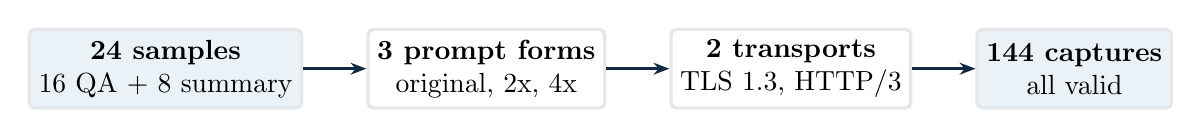
\begin{tikzpicture}[
    node distance=8mm,
    box/.style={rounded corners=2pt,draw=AIGrid,very thick,fill=white,
                minimum height=1.0cm,minimum width=2.45cm,align=center},
    arrow/.style={-{Stealth[length=2mm]},very thick,color=DeckNavy}
  ]
    \node[box,fill=DeckLight] (data) {\bfseries 24 samples\\16 QA + 8 summary};
    \node[box,right=of data] (compress) {\bfseries 3 prompt forms\\original, 2x, 4x};
    \node[box,right=of compress] (protocol) {\bfseries 2 transports\\TLS 1.3, HTTP/3};
    \node[box,right=of protocol,fill=DeckLight] (capture) {\bfseries 144 captures\\all valid};
    \draw[arrow] (data) -- (compress);
    \draw[arrow] (compress) -- (protocol);
    \draw[arrow] (protocol) -- (capture);
  \end{tikzpicture}

  \vspace{0.65cm}
  \begin{columns}[T,onlytextwidth]
    \column{0.32\textwidth}\centering
      {\bfseries Model}\\Qwen3.5-9B via vLLM
    \column{0.32\textwidth}\centering
      {\bfseries Determinism}\\temperature 0, seed 42
    \column{0.32\textwidth}\centering
      {\bfseries Network}\\loopback baseline
  \end{columns}
\end{frame}

\begin{frame}{Compression reaches distinct token budgets}
  \centering
  \PlotTokenMedians
  \vspace{-0.25cm}

  \small Median prompts shrink from 45.8k to 18.6k and 9.7k tokens for QA.
  \source{This experiment; medians across 16 QA and 8 summary samples.}
\end{frame}

\begin{frame}{QA upload falls by 54--76\%}
  \centering
  \PlotUploadReduction
  \vspace{-0.15cm}

  \small The reduction is nearly identical under TLS 1.3 and HTTP/3.
  \source{Paired medians; whiskers are deterministic bootstrap 95\% confidence intervals.}
\end{frame}

\begin{frame}{The workload determines total traffic savings}
  \centering
  \PlotTotalReduction
  \vspace{-0.15cm}

  \small QA gains survive end-to-end; summary gains are diluted by large generated responses.
  \source{Paired medians; bidirectional frame bytes.}
\end{frame}

\begin{frame}{QA is dominated by the uploaded prompt}
  \centering
  \PlotDirectionQA
  \vspace{-0.15cm}

  \small Compressing the input directly attacks the largest part of the exchange.
  \source{Median captured bytes; one run per sample-condition pair.}
\end{frame}

\begin{frame}{Generated summaries dominate bidirectional traffic}
  \centering
  \PlotDirectionSummary
  \vspace{-0.15cm}

  \small Upload shrinks, but response traffic remains roughly 220--255 KiB.
  \source{Median captured bytes; one run per sample-condition pair.}
\end{frame}

\begin{frame}{TLS and HTTP/3 carry similar total bytes}
  \centering
  \PlotProtocolBytes
  \vspace{-0.15cm}

  \small All median HTTP/3-to-TLS total-byte ratios remain within 4\% of parity.
  \source{Paired protocol ratios in a zero-RTT loopback baseline.}
\end{frame}

\begin{frame}{HTTP/3 packetization is visible on short exchanges}
  \centering
  \PlotProtocolPackets
  \vspace{-0.15cm}

  \small For original QA prompts, HTTP/3 uses 2.92x the captured packet count while transferring only 1.04x the bytes.
  \source{Paired medians; packet count includes all captured protocol traffic.}
\end{frame}

\begin{frame}{Latency follows the amount of input processed}
  \centering
  \PlotLatencyMedians
  \vspace{-0.15cm}

  \small QA falls from 8.6 s to 2.0 s at 4x; summary falls from 24.0 s to 20.8 s.
  \source{Median end-to-end generation latency; local model and loopback transport.}
\end{frame}

\begin{frame}{Three preliminary findings}
  \vspace{0.2cm}
  \begin{enumerate}
    \item[\color{AIBlue}\bfseries 01]\quad
      \textbf{Prompt tokens predict upload traffic.}
      Pearson $r=0.88$ for both transports.
    \vspace{0.35cm}
    \item[\color{AIOrange}\bfseries 02]\quad
      \textbf{Compression value is workload-dependent.}
      At 4x, median total traffic falls 71--73\% for QA but only 20--22\% for summaries.
    \vspace{0.35cm}
    \item[\color{AIGreen}\bfseries 03]\quad
      \textbf{Protocol choice changes packetization more than bytes.}
      TLS and HTTP/3 are close in total traffic and latency on loopback.
  \end{enumerate}
\end{frame}

\begin{frame}{Interpretation boundary and full-study plan}
  \begin{columns}[T,onlytextwidth]
    \column{0.47\textwidth}
      \begin{block}{What these results establish}
        \begin{itemize}
          \item end-to-end capture pipeline works
          \item compression levels are separable
          \item workload direction explains savings
          \item TLS and QUIC are directly comparable
        \end{itemize}
      \end{block}
    \column{0.47\textwidth}
      \begin{block}{Next controlled sweep}
        \begin{itemize}
          \item 52 workload items
          \item loopback and realistic RTT
          \item three repetitions
          \item controlled MTU and offloads
        \end{itemize}
      \end{block}
  \end{columns}
  \vspace{0.35cm}
  \centering
  {\Large\bfseries 52 $\times$ 3 $\times$ 2 $\times$ 2 $\times$ 3
   = \color{AIBlue}1,872 runs}
\end{frame}

\begin{frame}[standout]
  Prompt compression saves network traffic\\
  \textbf{when the prompt is the dominant payload.}

  \vspace{0.5cm}
  {\normalsize The next experiment tests whether this persists under realistic network conditions.}
\end{frame}

\begin{frame}{References and experiment artifacts}
  \small
  \begin{itemize}
    \item Pan et al. \emph{LLMLingua-2: Data Distillation for Efficient and Faithful Task-Agnostic Prompt Compression}. arXiv:2403.12968, 2024.
    \item Maharana et al. \emph{Evaluating Very Long-Term Conversational Memory of LLM Agents}. ACL 2024.
    \item Preliminary metrics: \texttt{artifacts/preliminary\_metrics\_baseline.csv}
    \item Reproducible figure pipeline: \texttt{analysis/prepare\_figure\_data.py}
  \end{itemize}
  \vspace{0.35cm}
  \footnotesize
  All numerical claims in this deck are computed from the 144 valid baseline captures.
\end{frame}

\end{document}
